Tramite uno script Python \`e stato possibile visualizzare determinati stati del sistema.
Per visualizzare al meglio la rete si \`e scelto di riportare i grafi relativi allo studio dei tempi di percorrenza.
Nel regime di traffico libero, cfr. Fig. \ref{fig:frequency_free_flow}, ci si aspetta che la quasi totalit\`a delle strade sia vuota.
\begin{figure}
    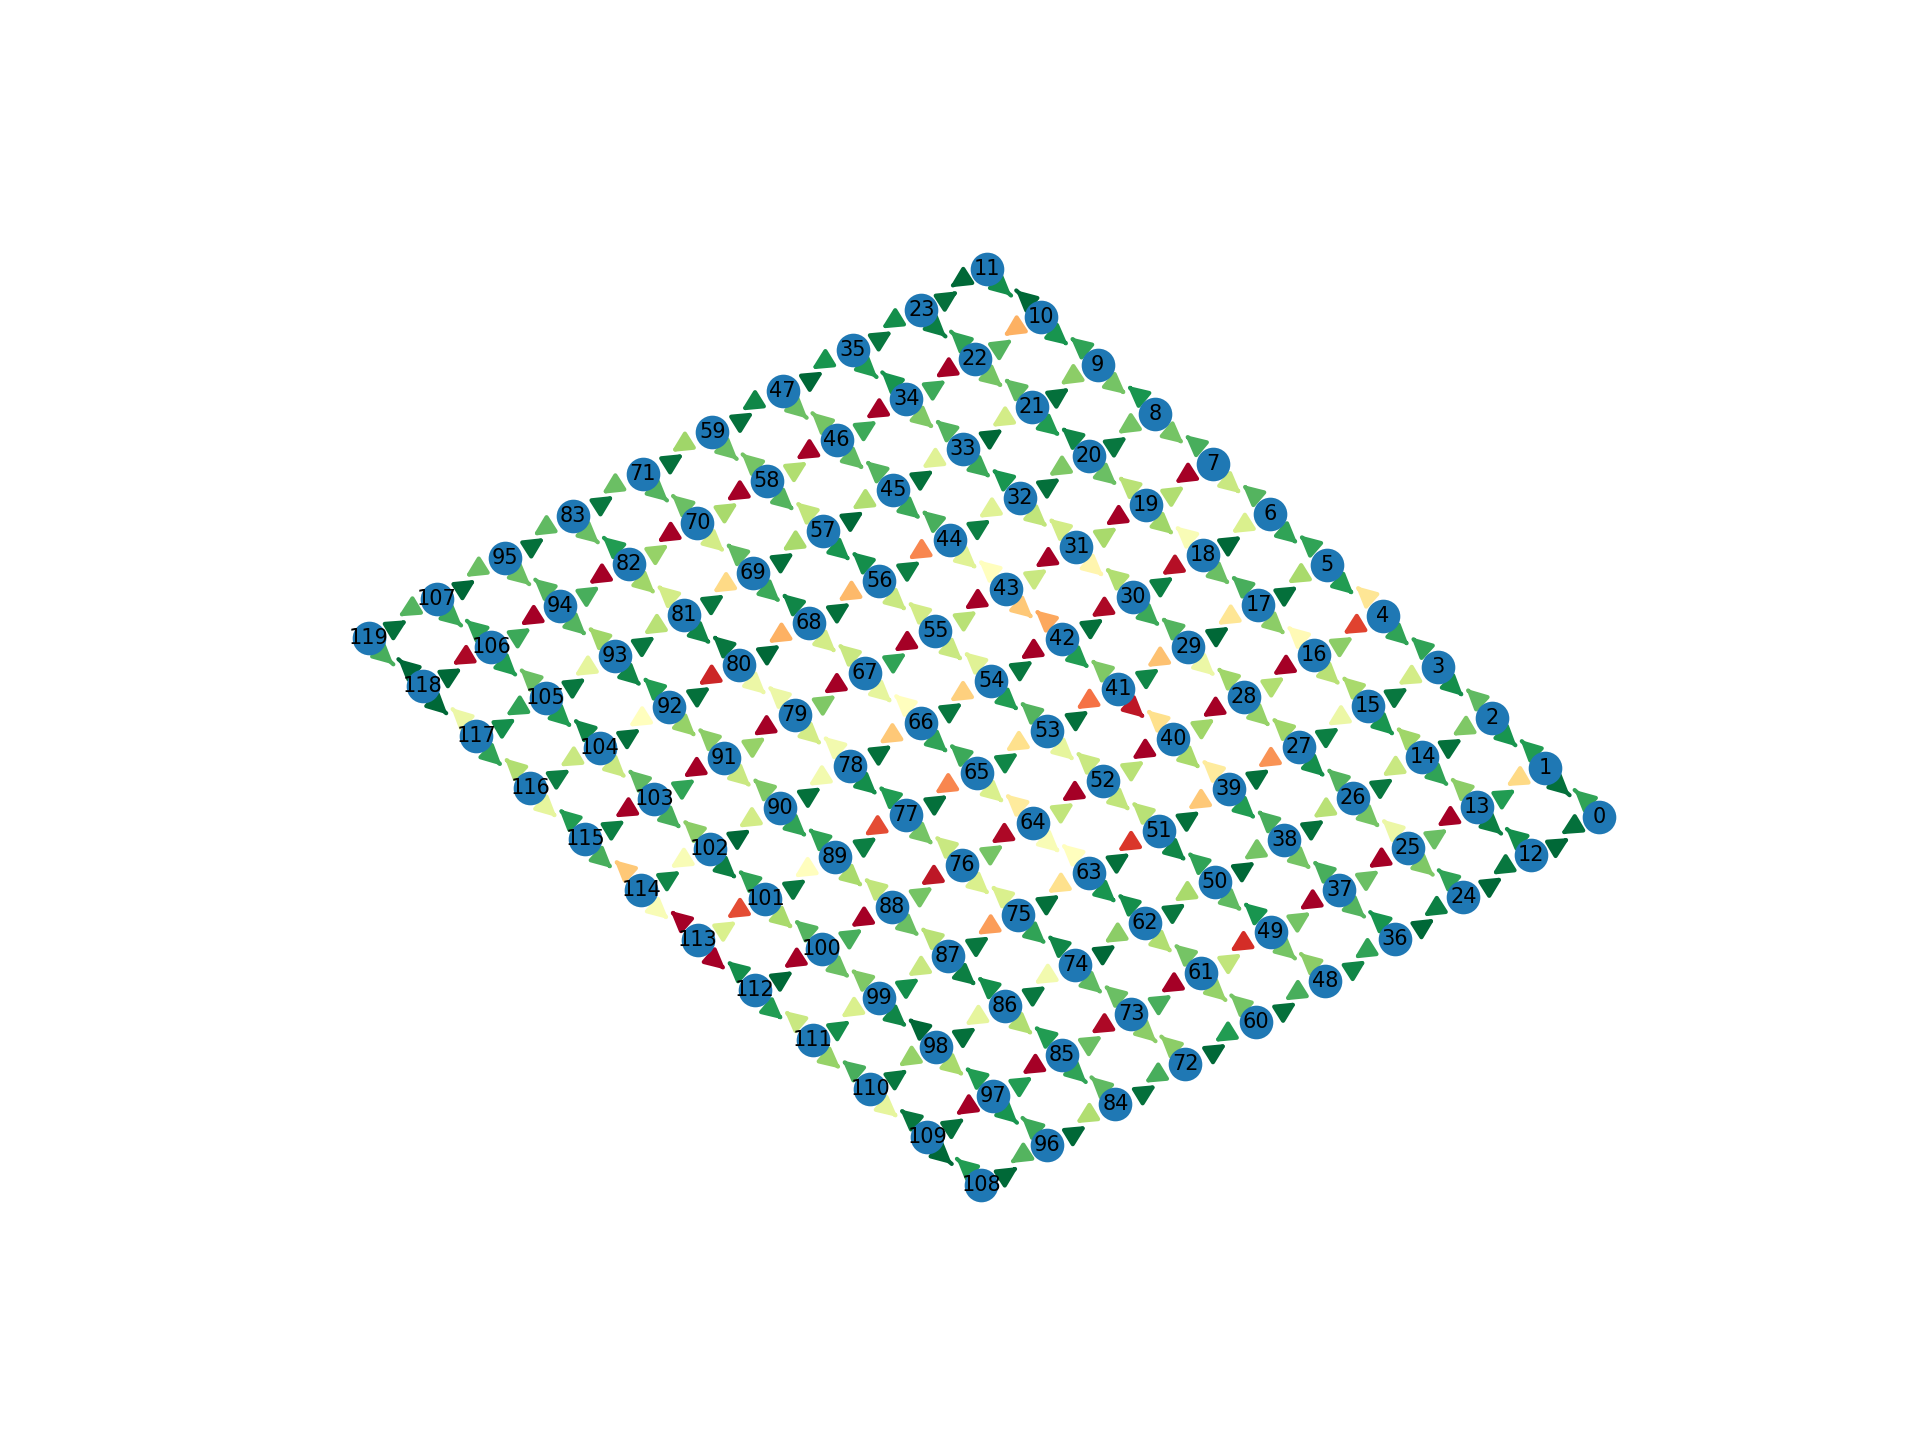
\includegraphics[scale=0.25, trim={2cm 5cm 10cm 5cm},clip]{./data/img/free_flow.png}
    \caption[Visualizzazione della rete non congestionata.]{\emph{Visualizzazione della rete non congestionata.}}
    \label{fig:visual_free}
\end{figure}
In Fig. \ref{fig:visual_free} si nota come gli unici percorsi congestionati, di colore rosso, siano le vie dirette dai nodi sorgenti alle destinazioni.
\begin{figure}
    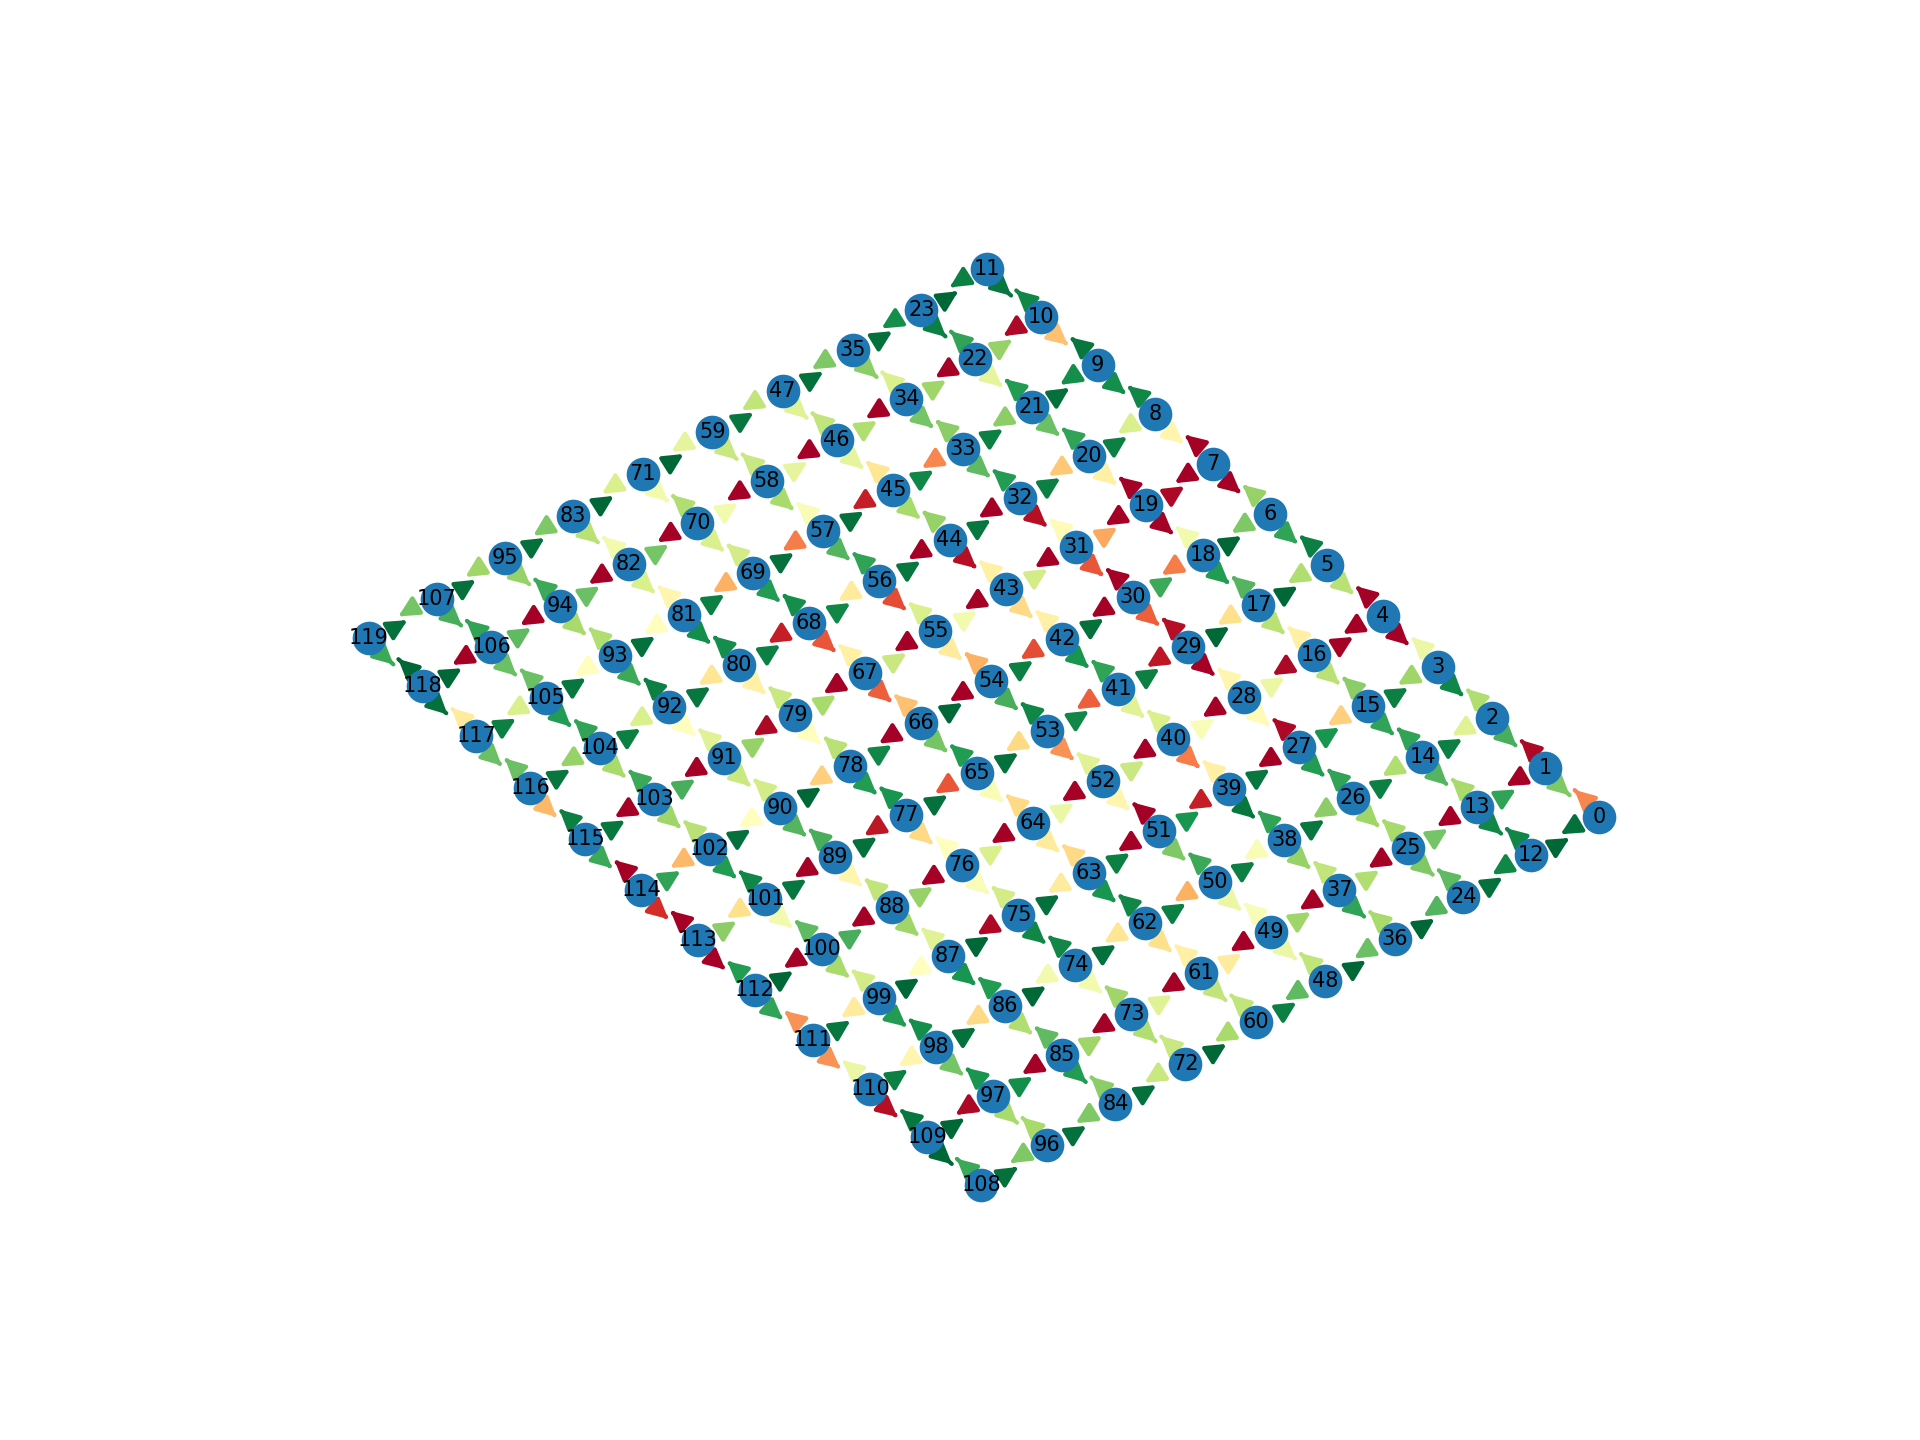
\includegraphics[scale=0.25, trim={2cm 5cm 10cm 5cm},clip]{./data/img/flow.png}
    \caption[Visualizzazione della rete mediamente congestionata.]{\emph{Visualizzazione della rete mediamente congestionata.}}
    \label{fig:visual_medium}
\end{figure}
In Fig. \ref{fig:visual_medium}, invece, il sistema comincia a entrare in congestione (cfr Fig. \ref{fig:frequency_flow}): si osservano cambiamenti nella densit\`a di veicoli sulle strade ortogonali ai percorsi diretti.
\begin{figure}
    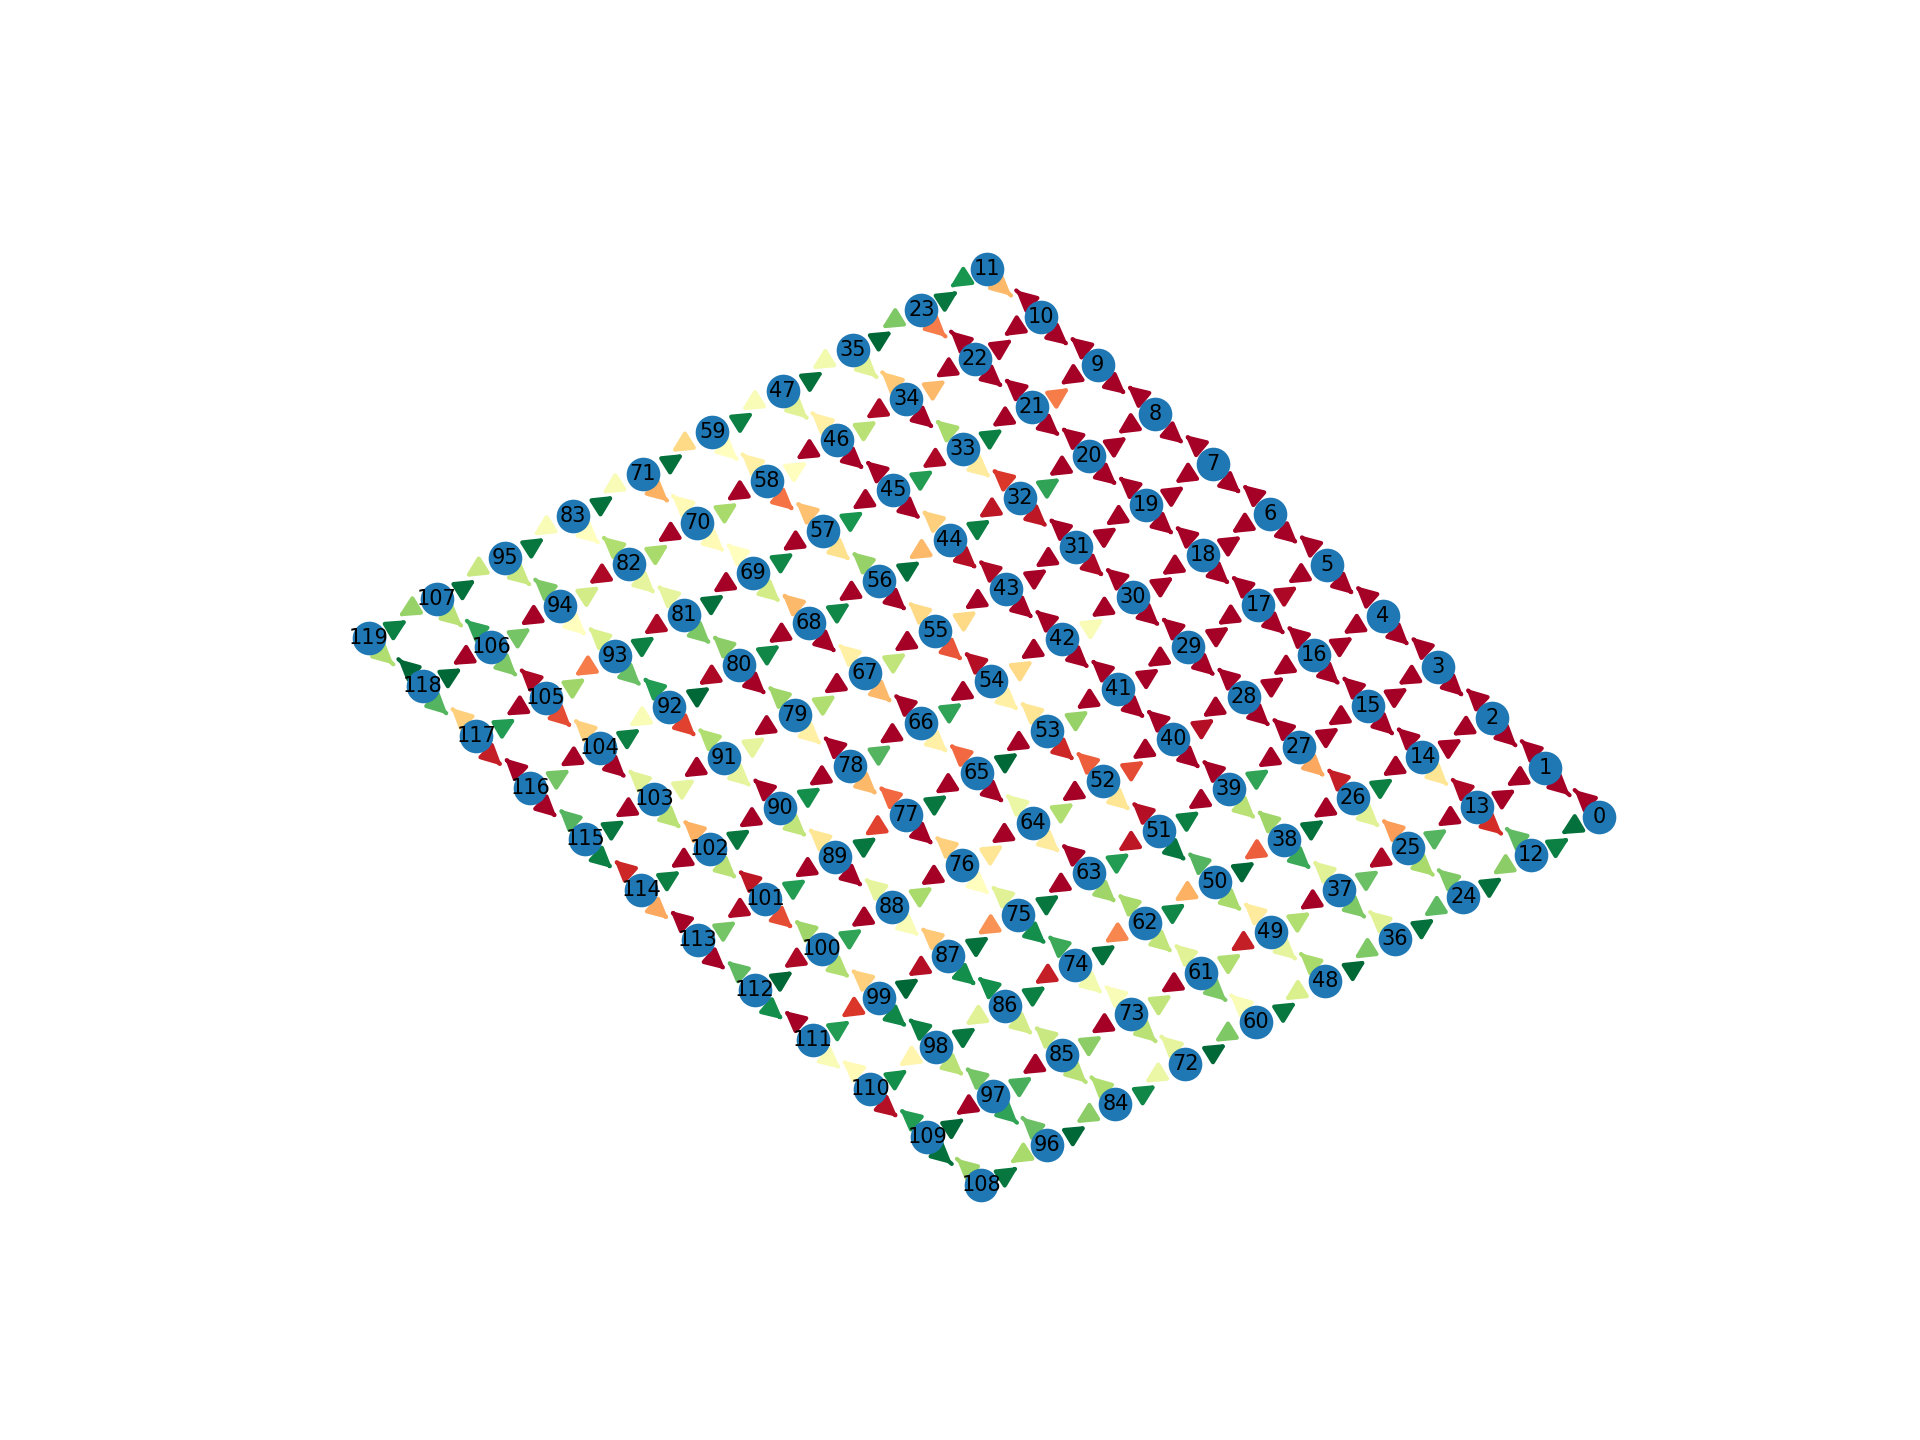
\includegraphics[scale=0.25, trim={2cm 5cm 10cm 5cm},clip]{./data/img/congested_flow.png}
    \caption[Visualizzazione della rete congestionata.]{\emph{Visualizzazione della rete congestionata.}}
    \label{fig:visual_congested}
\end{figure}
Infine, in Fig. \ref{fig:visual_congested} il sistema \`e congestionato e si ha una densit\`a di veicoli decisamente elevata in prossimit\`a dei nodi sorgente, cfr Fig. \ref{fig:frequency_congested_flow}.